% !TEX encoding = UTF-8
% !TEX program = lualatex
% Page Layout
\documentclass{beamer}
%\documentclass[beamer]
\usepackage{amssymb}

\let\Tiny=\tiny
\usepackage{tikz}
\usetikzlibrary{decorations.text}

\usepackage{chemfig}
\usepackage{siunitx}
\usepackage{graphicx}
\usepackage{url}
\usepackage[export]{adjustbox}
\usepackage{caption}
\usepackage{multirow}
\usepackage[T1]{fontenc}
\usepackage{fontspec,microtype}
\defaultfontfeatures{Ligatures=TeX, Scale=MatchLowercase}
\usepackage[german=quotes]{csquotes}
%\setmainfont[SmallCapsFeatures={LetterSpace=6}, Numbers={Proportional,OldStyle}]{Minion Pro}
%\setsansfont[LetterSpace=2, Numbers={Proportional,OldStyle}]{Myriad Pro}

\usepackage{array} % needed for \arraybackslash
\usepackage{tabularx}

\sisetup{
  round-mode          = places,
  round-precision     = 2,
  inter-unit-product =\ensuremath{{}\cdot{}}
}
 % Avoid an error due to a lack of registers

\definecolor{orange}{RGB}{255,127,0}
%\include{head}
\title[]{Alkaloiden}
\author[N. Arslan]{Nevroz Arslan}
\date[18.04.17]{18. Apr 2017}
%\titlegraphic{\includegraphics[width=\textwidth,height=.5\textheight]{bogen1200.png}}
\setbeamerfont{page number in head/foot}{size=\large}
\beamertemplatenavigationsymbolsempty


\let\otp\titlepage
\renewcommand{\titlepage}{\otp\addtocounter{framenumber}{-1}}

\renewcommand*\printatom[1]{\ensuremath{\mathsf{#1}}}


\definecolor{mygray}{RGB}{208,208,208}
\definecolor{mymagenta}{RGB}{226,0,116}
\newcommand*{\mytextstyle}{\sffamily\tiny\bfseries\color{black!85}}
\newcommand{\arcarrow}[3]{%
   % inner radius, middle radius, outer radius, start angle,
   % end angle, tip protusion angle, options, text
   \pgfmathsetmacro{\rin}{1.2}
   \pgfmathsetmacro{\rmid}{1.7}
   \pgfmathsetmacro{\rout}{2.2}
   \pgfmathsetmacro{\astart}{#1}
   \pgfmathsetmacro{\aend}{#2}
   \pgfmathsetmacro{\atip}{1}
   \fill[mygray, very thick] (\astart+\atip:\rin)
                         arc (\astart+\atip:\aend:\rin)
      -- (\aend-\atip:\rmid)
      -- (\aend:\rout)   arc (\aend:\astart+\atip:\rout)
      -- (\astart:\rmid) -- cycle;
   \path[
      decoration = {
         text along path,
         text = {|\mytextstyle|#3},
         text align = {align = center},
         raise = -1.0ex
      },
      decorate
   ](\astart+\atip:\rmid) arc (\astart+\atip:\aend+\atip:\rmid);
}

\newcommand{\arckarrow}[3]{%
   % inner radius, middle radius, outer radius, start angle,
   % end angle, tip protusion angle, options, text
   \pgfmathsetmacro{\rin}{1.2}
   \pgfmathsetmacro{\rmid}{1.7}
   \pgfmathsetmacro{\rout}{2.2}
   \pgfmathsetmacro{\astart}{#1}
   \pgfmathsetmacro{\aend}{#2}
   \pgfmathsetmacro{\atip}{1}
   \fill[mygray, very thick] (\astart+\atip:\rin)
                         arc (\astart+\atip:\aend:\rin)
      -- (\aend-\atip:\rmid)
      -- (\aend:\rout)   arc (\aend:\astart+\atip:\rout)
      -- (\astart:\rmid) -- cycle;
   \path[
      decoration = {
         text along path,
         text = {|\mytextstyle|#3},
         text align = {align = center},
         raise = -1.0ex,
         reverse path
      },
      decorate
   ](\astart+\atip:\rmid) arc (\astart+\atip:\aend+\atip:\rmid);
}


\newcommand{\arcyarrow}[3]{%
   % inner radius, middle radius, outer radius, start angle,
   % end angle, tip protusion angle, options, text
   \pgfmathsetmacro{\rin}{2.3}
   \pgfmathsetmacro{\rmid}{2.8}
   \pgfmathsetmacro{\rout}{3.2}
   \pgfmathsetmacro{\astart}{#1}
   \pgfmathsetmacro{\aend}{#2}
   \pgfmathsetmacro{\atip}{1}
   \fill[mygray, very thick] (\astart+\atip:\rin)
                         arc (\astart+\atip:\aend:\rin)
      -- (\aend-\atip:\rmid)
      -- (\aend:\rout)   arc (\aend:\astart+\atip:\rout)
      -- (\astart:\rmid) -- cycle;
   \path[
      decoration = {
         text along path,
         text = {|\mytextstyle|#3},
         text align = {align = center},
         raise = -1.0ex,
      },
      decorate
   ](\astart+\atip:\rmid) arc (\astart+\atip:\aend+\atip:\rmid);
}

\newcommand{\arcyrarrow}[3]{%
   % inner radius, middle radius, outer radius, start angle,
   % end angle, tip protusion angle, options, text
   \pgfmathsetmacro{\rin}{2.3}
   \pgfmathsetmacro{\rmid}{2.8}
   \pgfmathsetmacro{\rout}{3.2}
   \pgfmathsetmacro{\astart}{#1}
   \pgfmathsetmacro{\aend}{#2}
   \pgfmathsetmacro{\atip}{1}
   \fill[mygray, very thick] (\astart+\atip:\rin)
                         arc (\astart+\atip:\aend:\rin)
      -- (\aend-\atip:\rmid)
      -- (\aend:\rout)   arc (\aend:\astart+\atip:\rout)
      -- (\astart:\rmid) -- cycle;
   \path[
      decoration = {
         text along path,
         text = {|\mytextstyle|#3},
         text align = {align = center},
         raise = -1.0ex,
         reverse path
      },
      decorate
   ](\astart+\atip:\rmid) arc (\astart+\atip:\aend+\atip:\rmid);
}



\begin{document}
\makeatletter
\newenvironment{myitemize}{%
   \setlength{\topsep}{0pt}
   \setlength{\partopsep}{0pt}
   \renewcommand*{\@listi}{\leftmargin\leftmargini \parsep\z@ \topsep\z@ \itemsep\z@}
   \let\@listI\@listi
   \itemize
}{\enditemize}
\makeatother   


\setbeamercolor{block title}{use=structure,fg=black,bg=white}
\setbeamercolor{block body}{use=structure,fg=black,bg=white}
\setbeamerfont{frametitle}{size=\large}
%\usebackgroundtemplate{
%\includegraphics[width=1.0\paperwidth,height=0.17\paperheight]{bogen1200}
%\begin{tikzpicture}[overlay, remember picture]
%    \node[xshift=-10.80cm,yshift=1.15cm] at (0,0)    {\includegraphics[scale=0.6]{logo}};
%\end{tikzpicture}
%}


\addtobeamertemplate{frametitle}{\vskip+7ex}{}
\setbeamercolor{frametitle}{fg=black}
\setbeamertemplate{caption}{\insertcaption}

\setbeamertemplate{itemize/enumerate body begin}{\normalsize}
\setbeamerfont{frametitle}{size=\large}
\frame[plain]{\titlepage}
\defbeamertemplate{footline}{centered page number}
{%
 \hfill%
  \usebeamercolor[fg]{page number in head/foot}%
  \usebeamerfont{page number in head/foot}%
  \raisebox{.5cm}[0pt][0pt]{% <--- change here
    \insertframenumber\,/\,\inserttotalframenumber\kern1em}%
}

\setbeamertemplate{footline}[centered page number]
\setatomsep{3em}
\setdoublesep{4pt}

% tikz macro





\begin{frame}[t]{Sekundär Metaboliten}
\centering 
\begin{tikzpicture}
   \fill[even odd rule,mymagenta] circle (1);

   \node at (0,0) [
      font  = \mytextstyle,
      color = white,
      align = center
   ]{
      Photo-\\
      Synthese
   };
   \arckarrow{ 32 }{148 }{ Kohlenhydrat Metabolismus }
   \arcarrow{ 150 }{268}{ Stickstoff Metabolismus   }
   \arcarrow{ 270 }{390}{ Fettsäure Metabolismus    }
   \arcyrarrow{ 0 }{40}{ Flavonoide   }
   \arcyrarrow{ 41 }{82}{Chinone     }
   \arcyrarrow{ 83 }{110}{ Coumarine    }
   \arcyrarrow{ 111 }{141}{ Tanine    }
   \arcyrarrow{ 142 }{182}{ Glucosinolats    }
   \arcyarrow{ 183 }{243}{ Cyanogenglycoside   }
   \arcyarrow{ 244 }{284}{ Alkaloide    }
   \arcyarrow{ 285 }{325}{ Terpene    }
   \arcyarrow{ 326 }{359}{ Polyketide    }
 %  \arcarrow{250}{ 30}{ CHECK }
\end{tikzpicture}
\end{frame}



\begin{frame}[t]{Alkaloiden - Klassifizierung}
\begin{quote}
  Die \enquote{echten} Alkaloide werden nach den in ihnen enthaltenen
  heterocyclischen Ringsystemen eingeteilt.
\end{quote}
  \begin{table}[htpb]
    \tiny
    %\caption{Wichtige Gruppen der Alkaloide mit Aminosäurenvorstufen}
    \begin{tabular}{llll}
      \hline
      Strukturgruppe & Alkaloid Gruppe & Vorstufe & Beispiele \\
      \hline
      \chemfig[][scale=0.5]{
        =^[:270]% 2
        -[:330]% 3
        =^[:30]% 4
        -[:90]% 5
        (
        =^[:150]% 6
        -[:210]% -> 1
        )
        -[:30]% 7
        =_[:330]% 8
        -[:270]% 9
        =_[:210]N% 10
        (
        -[:150]% -> 4
        )
      }& Chinolin & Tryptophan & Chinin \\
      \multirow{3}{*}{\chemfig[][scale=0.5]{
        -[:300.8]N% 2
        -[:279.7]% 3
        -[:233.9,1.069]% 4
        -[:31.3,0.88]% 5
        -[:65.7,0.943]% 6
        (
        -[:141.9,0.864]\phantom{N}% -> 2
        )
        -[:1,1.126]% 7
        -[:279.6,1.005]% 8
        (
        -[:30,,,1]OH% 10
        )
        -[:140.3,0.813]% 9
        (
        -[:180,1.178]% -> 3
        )
    } } &  &  & Cocain \\
        & Tropan & Ornithin& Scopolamin\\
        && & Hyoscyamin\\
        &&&\\
        &&&\\
   \multirow{4}{*}{\chemfig[][scale=0.5]{
        R=[:0]% 6
       -[:300]% 5
       =^[:0]% 4
                 (
           -[:300]% 34
                     (
            -[:0,,,1]OH% 36
                     )
           =[:240]O% 35
                 )
    -[:60,,,1]NH% 3
    -[:120,,1]% 2
                 (
           -[:180]% 1
           -[:240]% -> 6
                 )
        <[:60]% 37
                 (
           =[:120]O% 38
                 )
    -[:0,,,1]OH% 39
    } } & Betalaine & Tyrosin & Betanidin \\
        && & Indicaxanthin\\
        &&&\\
        &&&\\
        &&&\\
        &&&\\
\multirow{4}{*}{\chemfig[][scale=0.5]{
    =^[:270]% 2
     -[:330]% 3
     =^[:30]% 4
      -[:90]% 5
               (
        =^[:150]% 6
         -[:210]% -> 1
               )
      -[:18]% 7
    =_[:306]% 8
     -[:234]\chembelow{N}{H}% 9
               (
         -[:162]% -> 4
               )
    } } & Indol & Tryptophan & Harmin \\
        && & Ergolin\\
        && & Strychinin\\
        && & Reserpin
    \end{tabular}
  \end{table}

\end{frame}
\begin{frame}[t]{Alkaloide - Klassifizierung}
   \begin{table}[htpb]
    \tiny
  %  \caption{Wichtige Gruppen der Alkaloide - II}
    \begin{tabular}{llll}
      \hline
      Strukturgruppe & Alkaloid Gruppe & Vorstufe & Beispiele \\
      \hline
      \multirow{3}{*}{\chemfig[][scale=0.5]{
    =^[:270]% 2
     -[:330]% 3
     =^[:30]% 4
     -[:330]% 5
     =^[:30]N% 6
      -[:90]% 7
    =^[:150]% 8
     -[:210]% 9
               (
         -[:270]% -> 4
               )
    =^[:150]% 10
               (
         -[:210]% -> 1
               ) 
    } } & Isochinolin & Tyrosin & Morphin \\
        && & Codein\\
        && & Papaverin\\
   \chemfig[][scale=0.5]{
       =^[:180]% 2
     -[:240]% 3
    =^[:300]N% 4
           -% 5
     =^[:60]% 6
               (
         -[:120]% -> 1
               )
    }  & Pyridin & Ornithin & Nicotin \\
\multirow{4}{*}{\chemfig[][scale=0.5]{
     =_[:330]% 2
     -[:270]% 3
               (
         -[:342]N% 7
         =^[:54]% 8
         -[:126]\chemabove{N}{H}% 9
         -[:198]% -> 2
               )
    =_[:210]N% 4
     -[:150]% 5
     =_[:90]N% 6
               (
          -[:30]% -> 1
               )
    } } & Purin & Glycin & Adenin \\
        && & Guanin\\
        && & Theobromin\\
        && & Coffein
    \end{tabular}
  \end{table}

 
\end{frame}
  \begin{frame}[t]{Alkaloide - weitere Einteilung}
    \begin{quote}
      Angehörige einer dieser Alkaloidgruppen können weiter nach am genannten
      Ringsystem ankondensierten zusätzlichen Ringen bestimmten Typen zuordnen. \footnotemark  
    \end{quote}
  
  \begin{columns}[onlytextwidth,t]
    \begin{column}{0.3\textwidth}
      \begin{minipage}[c][0.9\textheight][l]{\linewidth}
       \begin{figure}
    \centering
    \textbf{Ergolin}\par\medskip
        \includegraphics[height=2cm]{data/ergot/ergolingerust}% Place your graphic here
\end{figure} 
      \end{minipage}
    \end{column}
    \begin{column}{0.3\textwidth}
   \begin{minipage}[c][0.9\textheight][l]{\linewidth}
       \begin{figure}
    \centering
    \textbf{Ergolin-Typ}\par\medskip
        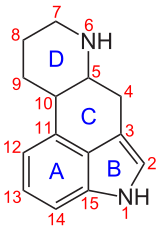
\includegraphics[height=2cm]{data/ergot/ergolinabcd}% Place your graphic here
\end{figure} 
      \end{minipage}
    \end{column}
   \begin{column}{0.3\textwidth}
      \begin{minipage}[c][0.9\textheight][l]{\linewidth}
     \begin{itemize}
       \item The base of ergot alkaloids is the tetracyclic ergoline ring
         system  
     \end{itemize}
      \end{minipage}
    \end{column}
  \end{columns}

\end{frame}

\begin{frame}[t]{Alkaloiden Typen}

  \begin{itemize}
    \item Indol Alkaloid-Typen: Strychinin, Yohimbin, $\beta$ - Carbolin,
      Physostigmin  ...
    \item Isochinolin-Typen: Morphinan-Typ (Morphin, Codein),
      Benzylisochinolin-Typ (Papaverin) (14 Typen)
    \item Tropanalkaloiden Typen:   
  \end{itemize}
  

\end{frame}

\begin{frame}[t]{Einteilung nach Vorkommen}
 
  \begin{table}[htpb]
    \centering
    %\caption{caption}
    %\label{tab:label}
    \begin{tabular}{llll}
      Familie & &Art & Alkaloide  \\
      Solanaceae & & Nicotina Rustica & Nicotin  \\
    \end{tabular}
  \end{table}
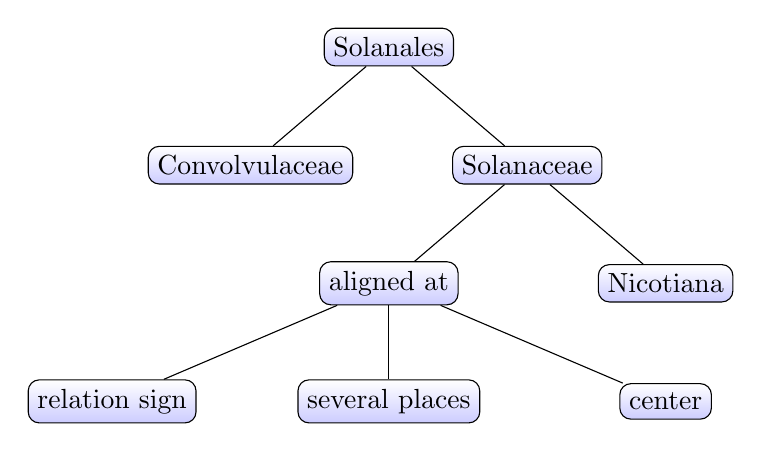
\begin{tikzpicture}[sibling distance=10em,
  every node/.style = {shape=rectangle, rounded corners,
    draw, align=center,
    top color=white, bottom color=blue!20}]]
  \node {Solanales}
    child { node {Convolvulaceae} }
    child { node {Solanaceae}
      child { node {aligned at}
        child { node {relation sign} }
        child { node {several places} }
        child { node {center} } }
      child { node {Nicotiana} } };
\end{tikzpicture}
\end{frame}


\begin{frame}[t]{Capsaicin}
  
\chemfig[][scale=0.5]{
     -[:270]% 2
               (
         -[:330]% 3
               )
     -[:210]% 4
     =[:150]% 5
     -[:210]% 6
     -[:150]% 7
     -[:210]% 8
     -[:150]% 9
     -[:210]% 10
               (
         =[:270]O% 11
               )
     -[:150]\chemabove{N}{H}% 12
     -[:210]% 13
     -[:150]% 14
    =_[:210]% 15
     -[:150]% 16
               (
         -[:210]O% 21
         -[:270]% 22
               )
     =_[:90]% 17
               (
     -[:150,,,2]HO% 20
               )
      -[:30]% 18
    =_[:330]% 19
               (
         -[:270]% -> 14
       )}
       \begin{itemize}
         \item Capsaicinoide sind farblos und sehr stabil. 
         \item Capsaicin bindet an den TRP-Kanal TRPV1, der auch durch eine Erhöhung der Temperatur aktiviert wird. Von diesem Umstand leitet sich der Ausdruck „brennen“ ab.
       \end{itemize}
       \url{https://de.wikipedia.org/wiki/Capsaicin}
\end{frame}

\begin{frame}[t,label=mohn]{Mohngewächse - Morphin Alkaloide - Isochinoilin Alkaloide }
  \begin{itemize}
    \item \textbf{Opium} wird als Rohopium aus den unreifen Fruchtkapseln des
      Schlafmohns und verwandter Arten gewonnen
    \item In unter anderem Gehirn und Rückenmark binden sie an Rezeptoren für
      \textbf{Endomorphine}
    \item schmerzlindernd, euphorisierende Wirkung
  \end{itemize}
  \begin{columns}[onlytextwidth,t]
    \begin{column}{0.6\textwidth}
      \begin{minipage}[c][0.9\textheight][l]{\linewidth}
        \begin{figure}
          \textbf{\tiny Papaver Somniferum}\par\medskip
        \includegraphics[height=3cm]{data/mohn/saft}% Place your graphic here
        \end{figure}
      \end{minipage}
   \end{column}
    \begin{column}{0.4\textwidth}
      \begin{minipage}[c][0.9\textheight][l]{\linewidth}
        \begin{figure}
          \textbf{\tiny Morphin}\par\medskip
        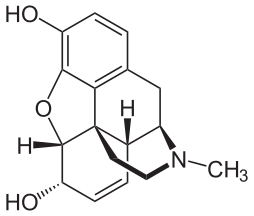
\includegraphics[height=3cm]{data/mohn/morphine}% Place your graphic here
        \end{figure}
      \end{minipage}
    \end{column}
  \end{columns}
  \end{frame}

  \begin{frame}[t]{Morphin-Alkaloide}
    \begin{itemize}
      \item Sie werden aus jeweils zwei Einheiten Tyrosin gebildet
    \end{itemize}

\begin{figure}

    \begin{tikzpicture}
      \node[label=Thebain] (thebain) at (-.5,0)[scale=0.2,draw=none]{
        \includegraphics{data/mohn/thebain}
      };
    \node[label=Codein] (codein) at (3,0)[scale=0.23,draw=none]{
        \includegraphics{data/mohn/codein}
      };
    \node[label=Morphin] (morphin) at (6.5,0)[scale=0.2,draw=none]{
        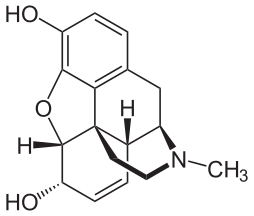
\includegraphics{data/mohn/morphine}
      };
    \draw [{Stealth}-{Stealth}] (thebain) -- (codein);
    \draw [{Stealth}-{Stealth}] (codein) -- (morphin);
    %\node [draw=red] (A) at (0,0) {1};
    %\node [draw=red] (B) at (2,0) {2};
  \end{tikzpicture}
\end{figure}


  \end{frame}

  \begin{frame}[t,label=schoellkraut]{Mohngewächse - Schöllkraut - Spartein }
    \begin{columns}[onlytextwidth,t]
      \begin{column}{0.6\textwidth}
        \begin{minipage}[c][0.9\textheight][l]{\linewidth}
          \begin{figure}
            \textbf{Schöllkraut}\par\medskip
            \includegraphics[height=3cm]{data/mohn/schoellkraut}% Place your graphic here
          \end{figure} 
        \end{minipage}
      \end{column}
      \begin{column}{0.4\textwidth}
        \begin{minipage}[c][0.9\textheight][l]{\linewidth}
          \begin{figure}
            \textbf{Spartein}\par\medskip
            \includegraphics[height=3cm]{data/mohn/sparteine}% Place your graphic here
          \end{figure} 
        \end{minipage}
      \end{column}
    \end{columns}
  \end{frame}


%\definesubmol{&}{-[,,,,draw=none]}
%\begin{frame}[t,label=tryptamin]
  \frametitle{Tryptophan}
  \schemestart
  \chemfig[][scale=0.35]{
            O% 13
     =[:282]% 12
               (
     -[:342,,,1]OH% 14
               )
     -[:222]% 11
               (
     <[:282,,,1]NH_2% 15
               )
     -[:162]% 10
     -[:222]% 7
     -[:168]% 5
     -[:240]% 4
               (
         -[:312]\chembelow{N}{H}% 9
          -[:24]% 8
         =^[:96]% -> 7
               )
    =_[:180]% 3
     -[:120]% 2
     =_[:60]% 1
           -% 6
               (
        =_[:300]% -> 5
               )
}
\arrow
\chemfig{X=[1]Y}\arrow
\chemfig{S>T}
\schemestop
	\end{frame}



%\begin{frame}[t,label=ephedraarten]
  \frametitle{Ephedra Arten}
  \begin{table}[htpb]
  %  \caption{caption}
    \begin{tabular}{cc}
      Ephedra monosperma & adsda  \\ 
    \end{tabular}
  \end{table}
\end{frame}



%\begin{frame}[t]
  \frametitle{Pseudoephedrin}
  \begin{itemize}
    \item Pseudoephedrin bewirkt vorwiegend in der Körperperipherie eine Ausschüttung von Katecholaminen \footnotemark 
    \item indirektes Sympathomimetikum
    \item Pseudoephedrin ist ein Phenylethylamin-Alkaloid 
    \item \chemfig[][scale=0.35]{*6(-=-(-(<:[2]OH)-[:-30](<:[6]CH_3)-[:30]N-[:-30])=-=)}
 
  \end{itemize}
  \footnotetext{\url{https://de.wikipedia.org/wiki/Pseudoephedrin}}
\end{frame}





\end{document}
